%%%%%%%%%%%%%%%%%%%%%%%%%%%%%%%%%%%%%%%%%%%%%%%%%%%%%%%%%%%%%%%%%%%%%%%%%%%%%%%%
%2345678901234567890123456789012345678901234567890123456789012345678901234567890
%        1         2         3         4         5         6         7         8

\documentclass[letterpaper, 10 pt, conference]{ieeeconf}  % Comment this line out
\usepackage[]{algorithm2e}      
\usepackage{xcolor} 
\newcommand\todo[1]{\textcolor{red}{#1}}                                     % if you need a4paper
%\documentclass[a4paper, 10pt, conference]{ieeeconf}      % Use this line for a4
                                                          % paper
\usepackage{graphicx}
\graphicspath{ {./images/} }
\IEEEoverridecommandlockouts                              % This command is only
                                                          % needed if you want to
                                                          % use the \thanks command
                                                          
                                                   
\overrideIEEEmargins
% See the \addtolength command later in the file to balance the column lengths
% on the last page of the document



% The following packages can be found on http:\\www.ctan.org
%\usepackage{graphics} % for pdf, bitmapped graphics files
%\usepackage{epsfig} % for postscript graphics files
%\usepackage{mathptmx} % assumes new font selection scheme installed
%\usepackage{times} % assumes new font selection scheme installed
%\usepackage{amsmath} % assumes amsmath package installed
%\usepackage{amssymb}  % assumes amsmath package installed

\title{\LARGE \bf
Attack Graph Generation for Micro-service
Architecture
}

%\author{ \parbox{3 in}{\centering Huibert Kwakernaak*
%         \thanks{*Use the $\backslash$thanks command to put information here}\\
%         Faculty of Electrical Engineering, Mathematics and Computer Science\\
%         University of Twente\\
%         7500 AE Enschede, The Netherlands\\
%         {\tt\small h.kwakernaak@autsubmit.com}}
%         \hspace*{ 0.5 in}
%         \parbox{3 in}{ \centering Pradeep Misra**
%         \thanks{**The footnote marks may be inserted manually}\\
%        Department of Electrical Engineering \\
%         Wright State University\\
%         Dayton, OH 45435, USA\\
%         {\tt\small pmisra@cs.wright.edu}}
%}

\author{Stevica Bozhinoski$^{1}$, Amjad Ibrahim$^{2}$ and Prof. Dr. Alexander Pretschner$^{3}$% <-this % stops a space
}

\begin{document}



\maketitle
\thispagestyle{empty}
\pagestyle{empty}



%%%%%%%%%%%%%%%%%%%%%%%%%%%%%%%%%%%%%%%%%%%%%%%%%%%%%%%%%%%%%%%%%%%%%%%%%%%%%%%%
\begin{abstract}
Microservices, in contrast to monolithic systems, provide an architecture that is modular and easily scalable. This advantage has resulted in a rapid increase in usage of microservices in recent years. Despite their rapid increase in popularity, there is a lack of work that focuses of their security aspect. Therefore, in the following paper, we present a novel Breath-First Search(BFS) based method for attack graph generation and security analysis of microservice architectures using Docker and Clair. 

\end{abstract}


%%%%%%%%%%%%%%%%%%%%%%%%%%%%%%%%%%%%%%%%%%%%%%%%%%%%%%%%%%%%%%%%%%%%%%%%%%%%%%%%
\section{INTRODUCTION}

\todo{We need to use the format of the conference, i added a folder ACM that contains it, please use it. And split the sections into different latex files using, so that we don't run into merges }

Attack graphs are a popular way of examining security aspects of network. They help security analysts to carefully analyse a system connection and detect the most vulnerable parts of the system. An attack graph depicts the actions that an attacker uses in order to reach his goal.  

 Statistics. They do not offer any performance comparison between different topologies. 

We first have a look into the work of other( Section 2), then present the architecure of our system(Section 3), test the scalability(Section 4) and at the end provide a conclusion(Section 5) and future work(Section 6).

\section{RELATED WORK}

Previous work has dealt with attack graph generation, mainly in computer networks \todo{please cite them}, where multiple machines are connected to each other and the Internet. In these networks an attacker performs multiple steps to achieve his goal, i.e., gaining privileges of a specific host. Attack graphs help in analyzing this behavior. Although attack graphs are useful, constructing them manually can be a cumbersome and time-consuming process\todo{elaborate a bit why; scalability, expertise, completeness.. }. Tools that generate vulnerabilities of specific host are available. However previous works have state that these tools alone are not enough to analyze the vulnerability \todo{mention why coz they can be connected ..} of an entire network and that these tools in addition to network topology could solve this issue. Therefore, some teams have been  working on developing systems that generate attack graphs automatically by using different approaches.

One of the earlier works in attack graph generation was done by Sheyner with using model checkers with goal property.\cite{ingols} \todo{space citation then the dot, e.g., property [5].}Model checkers use computational logic to check if a model is correct, and otherwise, they provide a counter example. A collection of these counter examples form an attack graph. They state that model checkers satisfy a monotonicity property in order to ensure termination. However model checkers have a computational disadvantage. In the example provided, NuSMV takes 2 hours to construct the attack graph with 5948 nodes and 68364 edges(Ingols reference) As a result of this, more scalable approach was needed. Amman et al. extends this work with some simplifications and more efficient storage.\cite{amman}

Ou et al. use logical attack graph\cite{ou} and Ingols\cite{ingols} et al. use breath first search algorithm in order to tackle the scalability issue. Ingols discusses the redundancy Full and Predictive graphs and model an attack graph as a MP graph with contentless edges and 3 types of nodes\todo{please rephrase this sentence to clarify it what is redundanccy full, define MP}. They use breath first search technique for generating the attack graph. This approach provides faster results in comparison to using model checkers. An MP graph of 8901 nodes and 23315 edges is constructed in 0.5 seconds.

Aksu et al. builds on top of Ingols's system and evaluate a set of rule pre- and postcondtions in generating attacks.\cite{aksu} They define a specific test of pre- and postcondition rules and test their correctness. In their evaluation, they use machine learning approach.

Containers and microservice architectures, despite their ever-growing popularity, have shown somewhat bigger security risks, mostly because of their bigger need of connectivity and lesser degree of encapsulation(Reference).To the best of our knowledge, there is no work that has been done so far in the area of attack graph generation for docker containers. Therefore we extend the work from Ingols\cite{ingols} and Aksu\cite{aksu} in conjuction to Clair OS to generate attack graphs for microservice architectures. Similar to computer networks, microservice architectures have a container topology and tools for analysis of containers. Containers in our model correspond to hosts, and a connection between hosts translates to a communication between containers. 
\todo{in general good story line, some language work is needed later-on}
\section{PROPOSED METHOD}


In this section we first have a look at Docker and attack graph terminology. We then present an overview of our proposed system with its components, provide a small example and at the end describe each of the components in more detail. 

\todo{it is early to put this image here, also long caption, image quality should be enhanced}
\begin{figure*}
	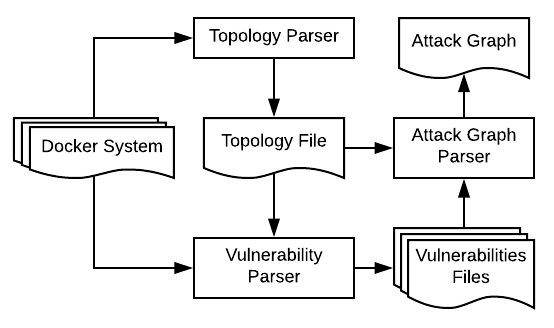
\includegraphics[width=\textwidth]{AttackGraphSystem}
	\caption{Our Attack Graph System. The rectangles denote the main components of the system: Topology Parser, Vulnerability Parser and Attack Graph Parser. The arrows describe the flow of the system and the files are the intermediate products.}
	\label{AttackGraphSystem}
\end{figure*}

In Docker, distinction is being made between the terms image, container and service. Image is an executable package that includes everything needed to run an application, container is a runtime instance of an image and service represents a container in production. A service only runs one image, but it codifies the way that image runs—what ports it should use, how many replicas of the container should run so the service has the capacity it needs, and so on. In our work we treat these terms equally, since we are doing a static and not runtime attack graph analysis.\cite{docker}

In this work we model an attack graph as a sequence of atomic attacks. Each atomic attack represents a transition from a component(with its privilege) to either the same component with a higher privilege or to a neighbor component with a new privilege. A goal of an attacker would be to perform multiple atomic attacks to reach the desired goal container. For example, let us suppose that an attacker wants to have access to a database of a certain website. In order to reach the database, he has to pass other containers between him and the database. He does that by finding a vulnerability to exploit and gives access to the container's neighbors. After a successful exploitation of multiple intermediate containers, he finally has access to the database and its content. Even though attack graphs model the attacker scenario from an attackers perspective, they are of crucial importance in computer security. For example, a system administrator would be interested to have an overview of the attack paths that an attacker could exploit, in order to harden the security of a given enterprise system.

Atomic attacks are fundamental building blocks in our attack graph. A single atomic attack represents a successful vulnerability exploitation. A consecutive sequence of atomic attacks represents a path in an attack graph and multiple attack paths constitute an attack graph. For an atomic attack to be executed, two constraints are imposed. First, the containers have to be connected between each other, so that physical access can be ensured. Second, the attacked container should contain some vulnerability that the attacker can exploit and gain a privilege level. We model the privileges into a hierarchy. The privileges in ascending order are: None, VOS(User), VOS(Admin), OS(User) and OS(Admin). VOS means that the privilege is connected to a virtual machine, while OS means that the host machine has been compromised. Since VOS are hosted on some machines, and their exploitation does not imply exploitation of the host machine, they are in the lower level of hierarchy.\cite{aksu}

Furthermore, in order for atomic attacks to be performed, certain preconditions have to be ensured. Preconditions are privilege levels that are required so that a vulnerability can be exploited. When an atomic attack is successfully executed, a postcondition is obtained. Postconditions are privileges acquired as a result of a successful attack. Both the Pre- and Postconditions are transformed from pre- and postcondition rules. We use in our attack graph generator the pre- and postconditions manually selected by experts and evaluated.\cite{aksu}

Nodes in our attack graph model are represented as a combination of a docker image and its respective privilege level, while edges are a connection between node pairs with the vulnerability that is being exploited as a descriptor. Once an attacker exploits a given vulnerability, he gains the privilege of the new container and an edge is added to the attack graph.

In order to show how the attack graph generation works in practice, we present a small example. The example is taken from the Netflix OSS Github repository.\cite{netflixoss} Displayed on figure \ref{TopologyGraph} is the topology of the example. The topology consists of "Outside" node, "Docker daemon" node and the a subset of other nodes. On figure \ref{AttackGraph}, we can see a part of the resulting attack graph. An example path than an attacker to take would be to first attack the Zuul container and gain USER privilege. Then with this USER privilege it can exploit another vulnerability to gain ADMIN privilege. Once the ADMIN privilege has been obtained on Zuul, the attacker can attack the Eureka container and gain ADMIN privilege. It is important to note that this is not the only path that the attacker can take in order to have ADMIN privileges on Eureka. Another path would be to use another Zuul vulnerability to gain directly ADMIN privileges and then attack the Eureka container.

Our attack graph generator is composed of three main components: Topology Parser, Vulnerability Parser and Attack Graph Parser(Fig. \ref{AttackGraphSystem}). The Topology Parser reads the underlying topology of the system and converts it into to a format needed for our Attack Graph Parser, the Vulnerability Parser generates the vulnerabilities for each of the images and the Attack Graph Parser generates the attack graph from the topology and vulnerabilities files. 

\begin{figure}
	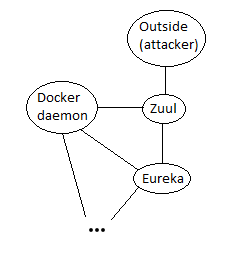
\includegraphics[]{Topology_graph}
	\caption{Example topology graph. The topology graph is a subset of a real topology graph from the Netflix OSS example. Each node denote container(plus Docker Deamon and Outside) and each edge denotes a connection between two containers.}
	\label{TopologyGraph}
\end{figure}

\begin{figure}
	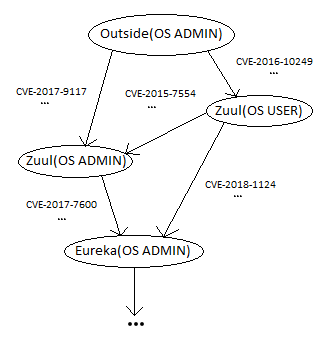
\includegraphics[]{Attack_graph}
	\caption{Example resulting attack graph. This attack graph is a subset of a real attack graph from the Netflix OSS example. Nodes correspond to a pair of container plus privilege, while edges are atomic attacks.}
	\label{AttackGraph}
\end{figure}


In the following subsections, we first have a look into the system requirements, then describe each of the parsers in more detail and finally examine the characteristics of the Breath-First Search graph transversal algorithm.

\subsubsection{Technical Details}
Our system is developed for Docker 17.12.1-ce and Docker Compose 1.19.0. The code is written in Python 3.6, and we use Clair\cite{clair} and Clairctl\cite{clairctl} for vulnerabilities generation.

We developed this system to be used exclusively with a specific version of Docker and Docker-Compose. However, please note that the main algorithm is easily extendable to accommodate other microservice architectures if the appropriate Topology and Vulnerability parsers are provided and conform to the input of the attack graph generator.

\subsubsection{Topology Parser}
The topology of Docker containers can be described at either runtime, or statically by using Docker Compose. In our case, since we are doing static attack graph analysis, we use Docker Compose as our main tool in the beginning. Docker Compose provides us with a docker-compose.yml file which is used for extraction of the topology of the system. However different versions of docker-compose.yml, use different syntax. For example older versions use the deprecated keyword "link", while newer ones use exclusively "networks", to denote a connection between two containers. In this work, we use the keyword "networks" as an indicator that a connection between two containers exists.

However, in the majority of cases, in order for an application to be useful, it has to communicate with the outside world. This is usually done using publishing ports. This is the case in both computer networks, as well as in microservice architectures.

Another consideration that we take into account is the privileged access. Some containers require certain privileges over the docker daemon in order to function properly. In docker this is usually done either by mounting the docker socket or specifying the keyword "privileged" in the docker-compose.yml file . An attacker with access to these containers, has also access to the docker daemon. Once the attacker has access to the docker daemon, he has potentially access to the whole microservice system, since every container is controlled and hosted by the daemon.





\begin{algorithm}
	\SetAlgoLined
	\KwData{topology, cont\_expl,
	priv\_acc}
	\KwResult{nodes, edges}
	nodes, edges, passed\_nodes = [], [], [] \\
	queue = Queue() \\
	queue.put("outside" + "ADMIN") \\

	\While{! queue.isEmpty()}{
		curr\_node = queue.get() \\
		curr\_cont = get\_cont(curr\_node) \\
		curr\_priv = get\_priv(curr\_node) \\
		neighbours = topology[curr\_cont] \\
	    \For{neigh in neighbours}{
	    	\If{curr\_cont == docker\_host}
	    	{
	    		end = neigh + "ADMIN" \\
	    		create\_edge(curr\_node, end) \\
	    		}
	        \If{neigh == docker\_host and priv\_acc[curr\_cont]}
	        { 	
	        	end = neigh + "ADMIN" \\
	        	create\_edge(curr\_node, end) \\
	        	queue.put(end) \\
	        	passed\_nodes.add(end)    	
	        	}
            \If{neigh != outside and neigh != docker\_host}{
            	precond = cont\_expl[neigh][precond] \\
            	postcond = cont\_expl[neigh][postcond] \\
            	\For{vul in vuls}{
            		\If{$curr_priv > precond[vul]$}{	
            	end = neigh + post\_cond[vul]\\
            	create\_edge(curr\_node, end\_node)\\
            	\If{end\_node not in passed\_nodes}{
            		queue.put(end\_node)\\
            		passed\_nodes.add(end\_node)
            		}}
            	}
                }
	    	}
	    nodes = update\_nodes()\\
	    edges = update\_edges() \\
	}

\caption{Breadth-first search algorithm for generating an attack graph.}
\label{BFSalgorithm}
\end{algorithm}

\begin{table*}
	\begin{center}
		\begin{tabular}{ |c|c|c|c|c|c|c|c| } 
			\hline
			Statistics & example\_1 & example\_5 & example\_20 & example\_50 & example\_100 & example\_500 & example\_1000 \\ 
			
			No. of Phpmailer containers & 1 & 1 & 1 & 1 & 1 & 1 & 1 \\ 
			
			No. of Samba containers & 1 & 5 & 20 & 50 & 100 & 500 & 1000 \\ 
			
			No. of nodes in topology & 4 & 8 & 23 & 53 & 103 & 503 & 1003\\ 
			
			No. of edges in topology & 6 & 28 & 253 & 1378 & 5253 & 126253 & 502503 \\ 
			
			No. nodes in attack graph & 5 & 13 & 43 & 103 & 203 & 1003 & 2003 \\ 
			
			No. edges in attack graph & 8 & 68 & 863 & 5153 & 20303 & 501503 & 2003003 \\ 
			
			Topology parsing time & 0.0082 & 0.0094 & 0.02879 & 0.0563 & 0.1241 & 0.7184 & 2.3664 \\ 
			
			Vulnerabilities preprocessing time & 0.2551 & 0.2840 & 0.5377 & 0.9128 & 1.6648 & 6.9961 & 15.0639 \\ 
			
			Breadth-First Search time & 0.0019 & 0.0209 & 0.2763 & 1.6524 & 6.5527 & 165.3634 & 767.5539 \\ 
			
			Total time & 0.2654 & 0.3144 & 0.8429 & 2.6216 & 8.3417 & 173.0781 & 784.9843 \\ 
			\hline
		\end{tabular}
	\end{center}
	
	\caption{Table with graph characteristics(no. of containers, nodes and edges in both the topology and attack graph) and executing times of the main attack graph generator components: Topology Parser, Vulnerability Preprocessing Module and Breadth-first Search Module(the latter two parts of the main attack graph generation process). The examples are composed of two containers: Phpmailer and Samba. The Phpmailer container has 181, while the Samba container has 367 vulnerabilities. The topology time is the time required to generate the graph topology. The vulnerabilities preprocessing time is the time required to convert the vulnerabilities into sets of pre- and postconditions. The Breath-First Search is the main component that generates the attack graph. All of the components are executed five times for each of the examples and their final time is averaged. The times are given in seconds. The total time contains the topology parsing, the attack graph generation and some minor processes. However, the total time does not include the vulnerability analysis by Clair. Evaluation of Clair can depend on multiple factors and it is therefore not in the scope of this analysis.}
	
	\label{table_scalability}
\end{table*}

\subsubsection{Vulnerability Parser}
In the preprocessing step, we use Clair to generate the vulnerabilities of a given container. Clair is a vulnerability scanner that inspects a docker image, and generate its vulnerabilities by providing CVE-ID, description and attack vector for each vulnerability. Attack vector is an entity that describes which conditions and effects are connected to this vulnerability. The fields in the attack vector as described by the National Vulnerability Database(NVD) are: Access Vector(Local, Adjacent Network and Network), Access Complexity(Low, Medium, High), Authentication(None, Single, Multiple), Confidentiality Impact(None, Partial, Complete), Integrity Impact(None, Partial, Complete) and Availability Impact(None Partial Complete). Although it is very useful, Clair does not provide with an easy to use interface to analyze a docker image. As a result, we use Clairctl(Clair wrapper) in order to analyze a complete docker image.


\subsubsection{Attack Graph Parser}
After the topology file is extracted and the vulnerabilities for each container are generated, we continue with the attack graph generation.

Here, we first preprocess the vulnerabilities and convert them into sets of pre- and postconditions. In order to do this, we match the attack vectors acquired earlier from the vulnerability database and keywords of the descriptions of each vulnerability to generate attack rules. When a subset of attack vector fields and description keywords matches a given rule, we use the pre- or postcondition of that rule. If more than one rule matches, we take the one with the highest privilege level for the preconditions and the lowest privilege level for the postconditions. If no rule matches we take None as a precondition and ADMIN(OS) as a postcondition. This results in a list of container vulnerabilities with their preconditions and postconditions.

\subsubsection{Breadth-First Search}

After the preprocessing step is done, the vulnerabilities are parsed and their pre- and postconditions are extracted. Together with the topology, they are feed into the Breadth-First Search algorithm(BFS).
Breadth-First Search is a popular search algorithm that traverses a graph by looking first at the neighbors of a given node, before going deeper in the graph. Pseudocode of our modified Breath First Search is given in Algorithm \ref{BFSalgorithm}. 

The algorithm requires a topology and a dictionary of the exploitable vulnerabilities as an input and the output is made up of nodes and edges that make the attack graph. 
The algorithm first initializes the nodes, edges, queue and the passed nodes. Afterwards it generates the nodes which are a combination of the image name and the privilege level.
Then into a while loop it iterates through every node, checks its neighbors and adds the edges if the conditions are satisfied. If the neighbor was not passed, then it is added to the queue. The algorithm terminates when the queue is empty. Furthermore BFS is characterized by the following properties:

\begin{itemize}
 \item Completeness: Breadth First Search is complete i.e. if there is a solution, breadth-first search will find it regardless of the kind of graph.
 \item Termination: This follows from its monotonicity property. Each edge is traversed only once.
 \item Time Complexity: is $O(|N| + |E|)$ where $|N|$ is the number of nodes and $|E|$ is the number of edges in the attack graph.
\end{itemize}


\section{EVALUATION}

In real-world microservice architectures, many containers are interconnected to each other. This raises the need for a scalable attack graph system. In this section, we first have a look at how others evaluate their systems. We then conduct few experiments in order to test the scalability of our system with different number of containers, and connections in both artificial and real networks. All of the experiments were performed on a Intel(R) Core(TM) i5-7200U CPU @ 2.50GHz with 8GB of RAM running Ubuntu 16.04.3 LTS.

Extensive scalability study of attack graph generators  is rare in current literature and many parameters contribute to the complexity of a comprehensive analysis. Characteristics that usually vary in this sort of evaluation are the number of nodes, their interconnectedness and the amount of vulnerabilities per container. All of these components contribute to the execution time of a given algorithm. Even though the definitions of an attack graph vary, we hope to reach a comprehensive comparison with current methods. In our case we compare our system to existing work by treating every container as a computer, and any physical connection between two computers as a connection between two containers. 

\begin{table*}
	\begin{center}
		\begin{tabular}{ |p{20mm}|p{25mm}|p{20mm}|p{10mm}|c|p{15mm}|p{45mm}| } 
			\hline
			Name & Description & Technology stack & No. Containers & No. vuln. & Attack Graph generation time & Github link \\\hline 
			
			Netflix OSS & Combination of containers provided from Netflix. & Spring Cloud, Netflix Ribbon, Spring Cloud Netflix, Netflix's Eureka & 10 & 4111 & 0.5120 sec. & https://github.com/Oreste-Luci/netflix-oss-example \\\hline
			
			Atsea Sample Shop App & An example online store application. & Spring Boot, React, NGINX, PostgreSQL & 4 & 120 & 0.2761 sec. & https://github.com/dockersamples/atsea-sample-shop-app \\\hline
			
			JavaEE demo & An application for browsing movies along with other related functions. & Java EE application, React, Tomcat EE & 2 & 149 & 0.2613 sec. & https://github.com/dockersamples/javaee-demo \\\hline
			
			PHPMailer and Samba & An artificial example created from two separate containers. We use an augmented version for the scalability tests. & PHPMailer(email creation and transfer class for PHP), Samba(SMB/CIFS networking protocol) & 2 & 548 & 0.2570 sec. & https://github.com/opsxcq/exploit-CVE-2016-10033
			https://github.com/opsxcq/exploit-CVE-2017-7494 \\\hline
			
			
			\hline
		\end{tabular}
	\end{center}
	
	\caption{List of randomly selected examples that were analyzed with our attack graph generation system.}
	\label{table_technologies}
	
\end{table*}

Seyner in his work tests the system in both a small and extended examples.\cite{sheyner} The attack graph in the larger example has 5948 nodes and 68364 edges. The time needed for NuSMV to execute this configuration is 2 hours, but the model checking part took 4 minutes. Sheyner claims that the performance bottleneck is inside the graph generation procedure. 

Ingols tested his system on a network of 250 hosts. He afterwards continued his study on a simulated network of 50000 hosts in under 4 minutes.\cite{ingols} Although this method yields better performance than the aforementioned approach, this evaluation is based on the Multiple Prerequisite graph, which is different from ours. In addition to this, missing explanation of how the hosts are connected, does not make it directly comparable to our method.

Ou provides some more extended study where he tests his system on more examples.\cite{ou}  He mentions that the asymptotic CPU time is between $O(n^2)$ and $O(n^3)$, where n is the number of hosts. The performance of the system for 1000 fully connected nodes takes more than 1000 seconds. He also provides an evaluation where he MulVAL clearly outperforms the Sheyner's system.

In our scalability experiments we use Samba\cite{samba} and Phpmailer\cite{phpmailer} containers which were taken from their respective Github repositories. We then extended this example and artificially made cliques of 5, 20, 50, 100, 500 and 1000 Samba containers to test the scalability of the system. The Phpmailer container has 181 vulnerabilities, while the Samba container has 367 vulnerabilities detected by Clair.

On Table \ref{table_scalability} we can see the results of our experiments. In each of these experiments the number of Phpmailer containers stays constant, while the number of Samba containers is increasing. This increase is done in a fully connected fashion, a node of each additional container is connected to every existing container. In addition, there are also two additional artificial containers("outside" that represents the environment from where the attacker can attack and the "docker host", i.e. the docker daemon where the containers are present). Therefore the number of nodes in the topology graph is the sum of: "outside", "docker host", number of Phpmailer containers and number of Samba containers. The number of edges of the topology graph is a a combination of: 1 edge("outside"-"Phpmailer"), n edges("docker host" to all of the containers) and clique of the Phpmailer and samba containers n*(n+1)/2. For example\_5, the number of containers would be 8(1 Phpmailer, 1 outside, 1 docker host and 5 Samba containers) the number of edges in the topology graph would be 32: 1 outside edge, 6 docker host edges(n=6, 1 Phpmailer and 5 Sambas) and 25 clique edges(5*6/2=15).

Throughout the experiments, for the smaller configurations, the biggest time bottleneck is the preprocessing step. However this step increases in linear fashion because the container files are analyzed only once by Clair. The attack graph generation for the smaller examples is considerably less than the preprocessing time. Starting from example\_500, we can notice sharp increase in BDF execution time to 165 seconds. For the previous example with example\_100, needed attack graph generation time is 6.5 seconds.

We also performed tests on some real examples as described on table \ref{table_technologies} and extend our system to different types of technologies, number of containers and vulnerabilities. The examples are as follows: NetflixOSS, Atsea Sample Shop App, and JavaEE demo. These examples are different from the synthetic ones presented above, since they contain less and different containers. They are connected in a more linear fashion in contrast to the full connection provided in the previous example. For example, in order for an attacker to reach a database, he needs to gain suitable privilege levels of multiple intermediate containers in several steps.



\section{CONCLUSION}

\section{FUTURE WORK}


\addtolength{\textheight}{-12cm}   % This command serves to balance the column lengths
                                  % on the last page of the document manually. It shortens
                                  % the textheight of the last page by a suitable amount.
                                  % This command does not take effect until the next page
                                  % so it should come on the page before the last. Make
                                  % sure that you do not shorten the textheight too much.

%%%%%%%%%%%%%%%%%%%%%%%%%%%%%%%%%%%%%%%%%%%%%%%%%%%%%%%%%%%%%%%%%%%%%%%%%%%%%%%%



%%%%%%%%%%%%%%%%%%%%%%%%%%%%%%%%%%%%%%%%%%%%%%%%%%%%%%%%%%%%%%%%%%%%%%%%%%%%%%%%



%%%%%%%%%%%%%%%%%%%%%%%%%%%%%%%%%%%%%%%%%%%%%%%%%%%%%%%%%%%%%%%%%%%%%%%%%%%%%%%%

\section*{ACKNOWLEDGMENT}





%%%%%%%%%%%%%%%%%%%%%%%%%%%%%%%%%%%%%%%%%%%%%%%%%%%%%%%%%%%%%%%%%%%%%%%%%%%%%%%%


\begin{thebibliography}{99}

\bibitem{docker} Merkel, Dirk. "Docker: lightweight linux containers for consistent development and deployment." Linux Journal 2014.239 (2014): 2.

\bibitem{clair}  CoreOS Clair. https://github.com/coreos/clair

\bibitem{clairctl}  Clairctl. https://github.com/jgsqware/clairctl

\bibitem{nvd}  Computer Security Division of National Institute of Standards and Technology.
National vulnerability database version 2.2 (2010),
http://nvd.nist.gov/

\bibitem{ingols}  Ingols, Kyle, Richard Lippmann, and Keith Piwowarski. "Practical attack graph generation for network defense." Computer Security Applications Conference, 2006. ACSAC'06. 22nd Annual. IEEE, 2006.

\bibitem{aksu}  Aksu, M. Ugur, et al. "Automated Generation Of Attack Graphs Using NVD." Proceedings of the Eighth ACM Conference on Data and Application Security and Privacy. ACM, 2018.

\bibitem{sheyner}  Sheyner, Oleg, et al. "Automated generation and analysis of attack graphs." Security and privacy, 2002. Proceedings. 2002 IEEE Symposium on. IEEE, 2002.

\bibitem{netspa}  Artz, Michael Lyle. Netspa: A network security planning architecture. Diss. Massachusetts Institute of Technology, 2002.

\bibitem{amman}  Ritchey, Ronald W., and Paul Ammann. "Using model checking to analyze network vulnerabilities." Security and Privacy, 2000. S\&P 2000. Proceedings. 2000 IEEE Symposium on. IEEE, 2000.

\bibitem{ou}  Ou, Xinming, Wayne F. Boyer, and Miles A. McQueen. "A scalable approach to attack graph generation." Proceedings of the 13th ACM conference on Computer and communications security. ACM, 2006.

\bibitem{samba} https://github.com/opsxcq/exploit-CVE-2017-7494

\bibitem{phpmailer} https://github.com/opsxcq/exploit-CVE-2016-10033

\bibitem{netflixoss} https://github.com/Oreste-Luci/netflix-oss-example
\end{thebibliography}




\end{document}
